Global Menu to funkcja pulpitu Ubuntu Unity, polegającą na przeniesieniu paska menu programu (\menu{Plik}, \menu{Edycja}, czy \menu{Narzedzia}) z okna programu na główny panel Unity (górny pasek menu). Po uruchomieniu dowolnej aplikacji, pasek menu zawiera jedynie nazwę aktualnie aktywnego okna:

\begin{center}
	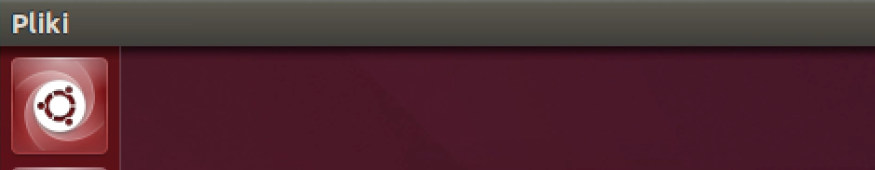
\includegraphics[width=\linewidth]{images/unity_menu_bar2.png}
\end{center}

Pasek menu jest aktywowany, gdy kursor myszy znajdzie się w jego obrębie:

\begin{center}
	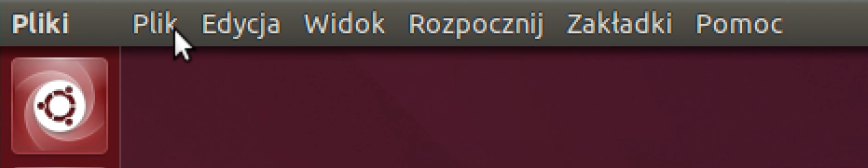
\includegraphics[width=\linewidth]{images/unity_menu_bar3.png}
\end{center}

Jeżeli korzystasz jedynie ze zmaksymalizowanych aplikacji, to Global Menu nie przeszkadza. Na ekranach panoramicznych lepiej jest wykorzystywane dostępne w pionie miejsce. Sprawa jednak się komplikuje, gdy korzystamy z okien w ich normalnym rozmiarze, a nie zmaksymalizowanych. Aby dostać się do menu, trzeba najpierw przesunąć kursor myszy na samą górę ekranu, a dopiero potem wybrać odpowiednią opcję. Na szczęście można to zmienić i zintegrować pasek narzędzi programu z belką tytułową aktywnego okna. 

Opcja ta jest dostępna poprzez:
\noindent \menu{{Ustawienia systemu}>{Wygląd}>{Zachowanie}>{Pokazuj menu okna}>{Na belce tytułowej okna}}.
